%% Chapter 3: Docker --- Architecture and Internals
%% Cybersecurity Lab Report --- Docker Escape via docker.sock Abuse and Command Injection

\chapter{Docker: Architecture and Internals}

%% ─────────────────────────────────────────────────────────────────────────────
\section{What Docker Is (and Is Not)}
%% ─────────────────────────────────────────────────────────────────────────────

Docker is frequently described as a lightweight virtualisation technology. This
description is misleading in a security context and must be corrected before the
attack surface can be accurately assessed. Docker performs no hardware emulation,
presents no virtual CPU, and runs no second kernel. It is, precisely, a toolchain
that automates the creation of namespaced process trees: it handles namespace
allocation, cgroup assignment, image unpacking, and process execution, and wraps all
of these operations behind a convenient command-line interface and a REST API.

The components that constitute the Docker system are:

\begin{itemize}
    \item \textbf{Docker CLI} (\texttt{docker}) --- a thin HTTP client that
          translates user commands into REST requests.
    \item \textbf{Docker daemon} (\texttt{dockerd}) --- the long-running, root-owned
          process that owns container lifecycle, image storage, networking, and
          volumes.
    \item \textbf{containerd} --- an industry-standard container runtime that manages
          lower-level lifecycle operations on behalf of \texttt{dockerd}.
    \item \textbf{runc} --- the OCI-compliant process launcher that makes the actual
          kernel calls to create namespaces and execute the container entrypoint.
\end{itemize}

A container, stripped of abstraction, is a namespaced and cgroup-limited process tree
executing on the host kernel. Docker adds value through its image format, registry
protocol, networking automation, volume management, and REST API surface. What it
does not add is a hardware isolation boundary.

The security implication is direct: because no hardware boundary exists, a kernel
vulnerability affects every container on the host simultaneously. More relevant to
this project, the Docker daemon (\texttt{dockerd}) runs as root on the host. It is
the privileged actor in the system---not the container. Any mechanism that grants a
container process the ability to communicate with the daemon is, in effect, a path to
host root.


%% ─────────────────────────────────────────────────────────────────────────────
\section{Docker vs Traditional Virtual Machines --- A Kernel-Level Comparison}
%% ─────────────────────────────────────────────────────────────────────────────

The distinction between virtual machine isolation and container isolation is not
merely a performance trade-off; it is a categorical difference in the security model.
Understanding this difference is essential to appreciating why the escape demonstrated
in this project requires no kernel exploit.

A virtual machine runs under a \textit{hypervisor}---either bare-metal (Type 1,
e.g., VMware ESXi, Xen) or hosted (Type 2, e.g., VirtualBox, QEMU/KVM). The
hypervisor emulates hardware, presenting a virtual CPU, memory bus, and devices to
the guest. The guest OS boots its own kernel in ring 0 of the virtual CPU. From the
guest's perspective, it owns dedicated hardware; from the host's perspective, the
guest is a managed process. Escaping a VM requires exploiting a vulnerability in the
hypervisor itself---typically a flaw in virtual device emulation (e.g., CVE-2015-3456
``VENOM'' in QEMU's floppy controller). Such vulnerabilities are rare, heavily
audited, and carry high exploitation complexity. Guest memory, CPU state, and devices
are fully virtualised: there is no shared kernel and no shared memory between guest
and host.

Container isolation, by contrast, rests entirely on kernel software primitives.
Namespaces restrict visibility; cgroups restrict resource consumption; capabilities
restrict privilege scope; seccomp and AppArmor narrow the syscall and file access
surface. All of these mechanisms were documented in Chapter~2. Because the host
kernel is shared, a container escape does not require defeating a hardware emulation
layer---it requires finding a misconfiguration or vulnerability in one of these
software mechanisms. The escape demonstrated in this project requires neither a
kernel CVE nor a seccomp bypass. It exploits a bind-mounted Unix socket and the
absence of daemon-side authentication, as established in Section~\ref{sec:dockersock}
and detailed in Chapter~4.

\begin{table}[h]
\centering
\caption{VM vs Container Isolation: Key Properties}
\label{tab:vm-vs-container}
\begin{tabular}{|l|l|l|}
\hline
\textbf{Property}       & \textbf{Virtual Machine}            & \textbf{Container}                  \\
\hline
Kernel                  & Separate per VM                     & Shared host kernel                  \\
Isolation boundary      & Hardware (hypervisor)               & Software (namespaces)               \\
Boot time               & Seconds to minutes                  & Milliseconds                        \\
Escape difficulty       & High (hypervisor CVE required)      & Lower (misconfiguration sufficient) \\
Syscall surface         & Virtualised                         & Direct to host kernel               \\
Overhead                & High (full OS stack)                & Near-zero                           \\
\hline
\end{tabular}
\end{table}

\begin{figure}[h]
\centering
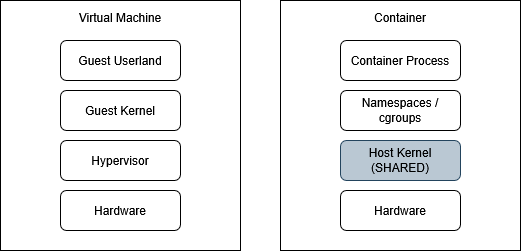
\includegraphics[width=0.9\textwidth]{images/ch3/isolation_stack.png}
% Diagram: VM vs Container Isolation Stack
% Side-by-side:
%   VM stack:        hardware → hypervisor → guest kernel → guest userland
%   Container stack: hardware → host kernel → namespaces → container process
% Highlight shared kernel on container side
\caption{VM vs Container Isolation Stack}
\end{figure}

The bottom row of Table~\ref{tab:vm-vs-container} encapsulates the attack in one
line: the syscall surface of a container is the host kernel's syscall table, not a
virtualised interface. Any process with access to the Docker daemon API bypasses this
comparison entirely---the daemon itself is a root process on the host that operates
outside all container isolation mechanisms.


%% ─────────────────────────────────────────────────────────────────────────────
\section{The Docker Daemon (\texttt{dockerd})}
\label{sec:dockerd}
%% ─────────────────────────────────────────────────────────────────────────────

\texttt{dockerd} is the privileged long-running process at the centre of the Docker
architecture. It owns every container lifecycle operation---creation, start, stop,
deletion---as well as image storage, network bridge management, and volume lifecycle.
It is not a container itself; it is a root-owned service running directly on the host
with an unrestricted capability set.

By default, \texttt{dockerd} listens for API requests on a Unix domain socket at
\texttt{/var/run/docker.sock}. Optionally, it can be configured to listen on a TCP
port, but the socket is always present in standard deployments. The socket's
permissions are:

\begin{lstlisting}[language=bash]
srw-rw---- 1 root docker
\end{lstlisting}

Ownership by the \texttt{docker} group means that any process whose effective UID is
0, or whose GID includes \texttt{docker}, may open the socket and issue API requests.
There is no further authentication mechanism: socket access is daemon-equivalent
power. This is the misconfiguration vector---when the socket is bind-mounted into a
container, the container process acquires the ability to issue commands to the daemon
as if it were a trusted local client.

\begin{lstlisting}[language=bash]
# Verify daemon is running as root
ps aux | grep dockerd

# Inspect socket file permissions
ls -la /var/run/docker.sock
# srw-rw---- 1 root docker

# Direct API call to daemon from the host
curl --unix-socket /var/run/docker.sock http://localhost/version
\end{lstlisting}

The daemon delegates actual container execution to \texttt{containerd} via a gRPC
channel on \texttt{/run/containerd/containerd.sock}. \texttt{dockerd} handles the
higher-level concerns---API parsing, image management, network configuration---and
instructs \texttt{containerd} to manage the runtime process lifecycle.

\begin{figure}[h]
\centering
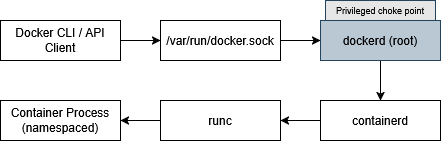
\includegraphics[width=0.9\textwidth]{images/ch3/docker_as_root_actor.png}
% Diagram: dockerd as Root Actor --- API Request Flow
% Shows: CLI → /var/run/docker.sock → dockerd (root) → containerd → runc → namespaced process
% Annotate: socket as the privileged choke point; dockerd runs as root on host
\caption{\texttt{dockerd} as Root Actor: API Request Flow}
\end{figure}

Because the daemon executes with full host-root privileges and performs its own
\texttt{clone()}, \texttt{mount()}, and \texttt{pivot\_root()} calls outside any
container's namespace or cgroup, none of the isolation mechanisms examined in
Chapter~2 constrain its actions. A caller that can reach the socket can instruct the
daemon to mount the host root filesystem into a new container and execute arbitrary
commands within it---as demonstrated in Chapter~8.


%% ─────────────────────────────────────────────────────────────────────────────
\section{containerd and runc}
%% ─────────────────────────────────────────────────────────────────────────────

Below \texttt{dockerd} sits a two-layer runtime stack whose separation clarifies
exactly where namespace creation and capability restriction occur.

\subsection{containerd}

\texttt{containerd} is a CNCF (Cloud Native Computing Foundation) container runtime
adopted as Docker's execution backend. It manages container lifecycle (create, start,
stop, delete), image storage via its snapshotter subsystem, and task supervision. It
communicates with \texttt{dockerd} over a gRPC channel on
\texttt{/run/containerd/containerd.sock}.

For each container, \texttt{containerd} spawns a \texttt{containerd-shim} process.
The shim is a lightweight supervisor that persists even if \texttt{containerd}
restarts: it holds the container's standard I/O streams, forwards exit codes, and
manages the \texttt{runc} lifecycle. Its persistence ensures containers are not
orphaned by daemon restarts.

\subsection{runc}

\texttt{runc} is the OCI-compliant low-level runtime. It is the component that
actually interacts with the kernel to create a container. Written in Go, \texttt{runc}
reads an OCI bundle (\texttt{config.json} plus a \texttt{rootfs/} directory) and
performs, in sequence:

\begin{itemize}
    \item \texttt{clone()} with namespace flags to create the process in fresh
          PID, NET, MNT, UTS, and IPC namespaces.
    \item \texttt{pivot\_root()} to switch the process's root filesystem to the
          container's OverlayFS mount.
    \item cgroup assignment by writing the process PID to the relevant cgroup
          \texttt{tasks} file.
    \item Capability bounding set reduction per \texttt{config.json}.
    \item \texttt{prctl(PR\_SET\_SECCOMP, ...)} to load the BPF filter.
    \item \texttt{execve()} to launch the container's entrypoint.
\end{itemize}

After \texttt{execve()} succeeds, \texttt{runc} exits. The \texttt{containerd-shim}
assumes supervision. The full execution chain is therefore:
\texttt{dockerd} $\rightarrow$ \texttt{containerd} $\rightarrow$
\texttt{containerd-shim} $\rightarrow$ \texttt{runc} $\rightarrow$ container PID 1.

\texttt{runc} has its own vulnerability history. CVE-2019-5736 allowed a malicious
container to overwrite the \texttt{runc} binary on the host via
\texttt{/proc/self/exe}, achieving a container escape without any misconfiguration.
The escape in this project requires no such exploit; it uses the daemon API directly.

\begin{lstlisting}[language=bash]
# Observe containerd and shim processes on the host
ps aux | grep containerd

# Low-level runc management
runc list
runc state <container-id>

# containerd socket permissions
ls -la /run/containerd/containerd.sock
\end{lstlisting}

\begin{figure}[h]
\centering
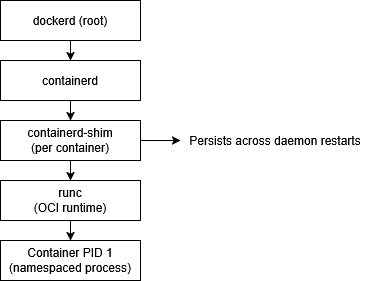
\includegraphics[width=0.6\textwidth]{images/ch3/docker_runtime_stack.png}
% Diagram: Docker Runtime Stack --- dockerd → containerd → runc → Process
% Full call chain with process names and IPC sockets between layers
% Annotate where clone() syscall fires (at runc level)
\caption{Docker Runtime Stack: \texttt{dockerd} $\rightarrow$ \texttt{containerd} $\rightarrow$ \texttt{runc} $\rightarrow$ Process}
\end{figure}


%% ─────────────────────────────────────────────────────────────────────────────
\section{The OCI Runtime Specification}
%% ─────────────────────────────────────────────────────────────────────────────

The Open Container Initiative (OCI), a Linux Foundation project, defines two
interoperable standards: the \textit{Runtime Specification}, which describes how a
compliant runtime must create and manage a container, and the \textit{Image
Specification}, which describes how a container image must be packaged and layered.
Any OCI-compliant runtime---\texttt{runc}, \texttt{crun}, or Kata Containers'
\texttt{kata-runtime}---can execute an OCI bundle.

An OCI bundle consists of a \texttt{config.json} file and a \texttt{rootfs/}
directory. \texttt{config.json} is the contract between the caller and the runtime.
The fields most relevant to security are:

\begin{itemize}
    \item \textbf{\texttt{namespaces}} --- the list of namespace types to create for
          this container (PID, NET, MNT, etc.).
    \item \textbf{\texttt{capabilities}} --- the permitted, effective, and bounding
          sets that the container process will hold after startup.
    \item \textbf{\texttt{seccomp}} --- the BPF filter profile to load.
    \item \textbf{\texttt{mounts}} --- the list of bind mounts to apply, including
          any \texttt{docker.sock} entries introduced by \texttt{-v} flags.
    \item \textbf{\texttt{linux.devices}} --- device nodes to expose inside the
          container; expanded by \texttt{--privileged}.
\end{itemize}

When a user passes \texttt{-v /var/run/docker.sock:/var/run/docker.sock} to
\texttt{docker run}, Docker translates this flag into a mount entry in
\texttt{config.json} before handing the bundle to \texttt{runc}. The entry appears
as:

\begin{lstlisting}[language=bash]
{
  "destination": "/var/run/docker.sock",
  "source":      "/var/run/docker.sock",
  "options":     ["rbind", "rprivate"]
}
\end{lstlisting}

This JSON fragment is the root cause of the misconfiguration. \texttt{runc} reads
it and calls \texttt{mount(MS\_BIND)} to attach the host socket path into the
container's mount namespace. The OCI bundle for a running container can be inspected
directly:

\begin{lstlisting}[language=bash]
cat /run/containerd/io.containerd.runtime.v2.task/moby/<id>/config.json
# reveals full namespace list, capability sets, seccomp profile, and mounts
\end{lstlisting}


%% ─────────────────────────────────────────────────────────────────────────────
\section{How \texttt{docker run} Becomes a Process --- Full Syscall Flow}
\label{sec:dockerrun-flow}
%% ─────────────────────────────────────────────────────────────────────────────

Tracing the complete path from \texttt{docker run} to a running namespaced process
reveals precisely where each kernel primitive from Chapter~2 is applied. The sequence
is as follows.

First, the Docker CLI parses the command-line flags and constructs an HTTP POST
request to the \texttt{/containers/create} endpoint on \texttt{dockerd}, transmitted
over \texttt{/var/run/docker.sock}. Second, \texttt{dockerd} receives the request,
pulls the image if it is not locally cached, and generates an OCI bundle including a
\texttt{config.json} encoding all runtime parameters. Third, \texttt{dockerd} calls
\texttt{containerd} over gRPC (\texttt{containerd.TaskService.Create}). Fourth,
\texttt{containerd} spawns a \texttt{containerd-shim-runc-v2} process. Fifth, the
shim invokes \texttt{runc run}.

Sixth---and most important for the kernel model---\texttt{runc} reads
\texttt{config.json} and executes the following sequence of syscalls:

\begin{itemize}
    \item \texttt{clone(CLONE\_NEWPID | CLONE\_NEWNS | CLONE\_NEWNET |} \\
          \texttt{CLONE\_NEWUTS | CLONE\_NEWIPC)} --- allocates fresh namespaces for
          the container process.
    \item \texttt{unshare(CLONE\_NEWUSER)} --- if user namespace remapping is
          enabled; not present in the default configuration used in this project.
    \item \texttt{pivot\_root()} --- switches the container process's root filesystem
          to the OverlayFS merged mount, replacing the host \texttt{/}.
    \item cgroup assignment --- the container's PID is written to the appropriate
          cgroup \texttt{tasks} file, applying resource limits.
    \item Capability drop --- the bounding set is reduced by clearing bits via
          \texttt{prctl(PR\_CAPBSET\_DROP)}.
    \item \texttt{prctl(PR\_SET\_SECCOMP, SECCOMP\_MODE\_FILTER, ...)} --- loads the
          BPF filter specified in \texttt{config.json}.
    \item Bind mounts (including \texttt{docker.sock}) are applied via
          \texttt{mount(MS\_BIND)} after \texttt{pivot\_root}.
    \item \texttt{execve()} --- replaces the \texttt{runc} process image with the
          container entrypoint (e.g., \texttt{python3 app.py}).
\end{itemize}

After \texttt{execve()}, \texttt{runc} exits and the \texttt{containerd-shim}
supervises the resulting container PID 1. From this moment, the container process is
running inside its namespace set with the bind-mounted \texttt{docker.sock} live in
its filesystem. The socket is present before the application code begins executing.

The syscall sequence can be observed live:

\begin{lstlisting}[language=bash]
strace -f -e clone,unshare,mount,pivot_root,execve \
  docker run --rm alpine echo hi 2>&1 | head -40
\end{lstlisting}

The HTTP layer can also be exercised directly, bypassing the CLI:

\begin{lstlisting}[language=bash]
curl --unix-socket /var/run/docker.sock \
  -X POST "http://localhost/containers/create" \
  -H "Content-Type: application/json" \
  -d '{"Image":"alpine","Cmd":["sh"]}'
\end{lstlisting}

This direct API interaction is the technique used in the escape chain: a
\texttt{curl} or \texttt{docker} binary inside the container issues the same HTTP
request, but the socket it reaches is the host daemon's socket, not a sandboxed
proxy.


%% ─────────────────────────────────────────────────────────────────────────────
\section{Docker Images and Layers (OverlayFS)}
%% ─────────────────────────────────────────────────────────────────────────────

A Docker image is an ordered, immutable stack of filesystem layers. Each layer is
a \texttt{tar} archive encoding the filesystem diff produced by a single
\texttt{Dockerfile} instruction (\texttt{RUN}, \texttt{COPY}, \texttt{ADD}, etc.).
Layers are stored on the host under \texttt{/var/lib/docker/overlay2/} and are
shared across containers that derive from the same base image.

At runtime, Docker assembles these layers into a unified filesystem view using
\textbf{OverlayFS}:

\begin{itemize}
    \item \textbf{\texttt{lowerdir}} --- the read-only stack of image layers,
          ordered from base to most recent.
    \item \textbf{\texttt{upperdir}} --- a per-container writable layer; all writes
          from within the container land here.
    \item \textbf{\texttt{workdir}} --- OverlayFS's internal staging area, required
          by the kernel implementation.
    \item \textbf{\texttt{merged}} --- the unified view presented as the container's
          root filesystem (\texttt{/}).
\end{itemize}

OverlayFS implements copy-on-write: reads are served from \texttt{lowerdir} until a
file is modified, at which point it is copied into \texttt{upperdir} and the write
applied there. When a container is deleted, \texttt{upperdir} is discarded; the image
layers in \texttt{lowerdir} remain intact and available to future containers.

A bind mount (\texttt{-v}) bypasses the OverlayFS stack entirely. It is implemented
as a \texttt{mount(MS\_BIND)} syscall that maps a host path directly into the
container's merged view. The \texttt{docker.sock} bind mount is not part of any image
layer; its inode lives on the host filesystem and is made accessible inside the
container without being copied, cached, or mediated by OverlayFS. The socket is
identical on both sides of the mount namespace boundary, as established in
Section~\ref{sec:mountns}.

\begin{lstlisting}[language=bash]
# View active OverlayFS mounts for running containers
mount | grep overlay

# Inspect layer paths via Docker inspect
docker inspect netdiag-app | python3 -c \
  "import sys,json; d=json.load(sys.stdin); \
   [print(g) for g in d[0]['GraphDriver']['Data'].values()]"

# Host overlay directory structure
ls /var/lib/docker/overlay2/
\end{lstlisting}


%% ─────────────────────────────────────────────────────────────────────────────
\section{Docker Networking Internals (Bridge, iptables, veth Pairs)}
%% ─────────────────────────────────────────────────────────────────────────────

Docker's default network mode is \texttt{bridge}. On first use, Docker creates a
virtual bridge interface \texttt{docker0} on the host with IP address
\texttt{172.17.0.1} and subnet \texttt{172.17.0.0/16}. Each container that joins
the default bridge network is connected to it via a \textit{virtual Ethernet pair}
(\texttt{veth}): a kernel-level point-to-point link whose two ends behave as ordinary
Ethernet interfaces.

One end of the veth pair (\texttt{vethXXXXXX}) is attached to \texttt{docker0} on
the host; the other end (\texttt{eth0}) is placed inside the container's network
namespace and assigned an IP address from Docker's IPAM pool (e.g.,
\texttt{172.17.0.2}). Traffic leaving the container traverses this path:
container \texttt{eth0} $\rightarrow$ veth pair $\rightarrow$ \texttt{docker0} bridge
$\rightarrow$ host NIC, with Network Address Translation applied by an iptables
\texttt{MASQUERADE} rule in the \texttt{POSTROUTING} chain.

Port mapping (e.g., \texttt{-p 5000:5000}) is implemented by \texttt{dockerd} as an
iptables DNAT rule in the \texttt{PREROUTING} chain, rewriting the destination
address of packets arriving on host port 5000 to the container's IP and port. A
corresponding \texttt{FORWARD} rule permits the bridged traffic.

For the reverse shell documented in Chapter~8, the relevant traffic path is: shell
process inside container $\rightarrow$ TCP connect to attacker IP on port 4444
$\rightarrow$ kernel TCP stack $\rightarrow$ \texttt{eth0} $\rightarrow$ veth pair
$\rightarrow$ \texttt{docker0} $\rightarrow$ iptables \texttt{MASQUERADE} $\rightarrow$
host NIC $\rightarrow$ NAT network $\rightarrow$ attacker VM. No elevated network
privilege is required for this path; outbound TCP connections are permitted under the
default network namespace configuration.

The flag \texttt{--network=host} removes the network namespace entirely, placing the
container directly on the host's network stack. This is a separate misconfiguration
not present in the lab environment.

\begin{figure}[h]
\centering
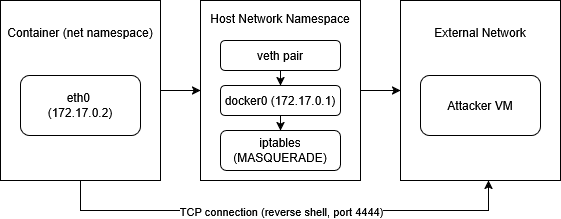
\includegraphics[width=0.9\textwidth]{images/ch3/docker_run.png}
% Diagram: Docker Bridge Networking --- Container to Host to External
% Shows: Container eth0 → veth pair (kernel) → docker0 bridge → iptables NAT → host NIC → external
% Annotate reverse shell traffic direction with a labelled arrow
% Include DNAT rule annotation for port 5000
\caption{Docker Bridge Networking: Container to Host to External Network}
\end{figure}

\begin{lstlisting}[language=bash]
# View docker0 bridge and attached veth pairs
ip link show
brctl show docker0

# iptables NAT rules added by Docker
iptables -t nat -L -n -v | grep -E "DOCKER|DNAT|MASQ"

# Container's network view
docker exec netdiag-app ip addr
docker exec netdiag-app ip route
\end{lstlisting}


%% ─────────────────────────────────────────────────────────────────────────────
\section{Docker Volumes and Bind Mounts}
\label{sec:bindmounts}
%% ─────────────────────────────────────────────────────────────────────────────

Docker offers two mechanisms for persisting or sharing data between host and
container: managed volumes and bind mounts. Their kernel-level behaviour differs
substantially, and the difference is the foundation of the misconfiguration exploited
in this project.

\subsection{Docker Volumes}

A Docker volume is managed entirely by \texttt{dockerd}. Volumes are stored under
\texttt{/var/lib/docker/volumes/} and are mounted into containers via
\texttt{mount(MS\_BIND)} from that daemon-controlled path. Their lifecycle is tied to
the Docker object model rather than to any specific host filesystem path, making them
the safer default: they expose no arbitrary host directory to the container.

\subsection{Bind Mounts}

A bind mount (\texttt{-v /host/path:/container/path}) instructs the kernel to make a
specific host path visible at a second location via a direct \texttt{mount(MS\_BIND,
host\_path, container\_path)} syscall. The host path's inode is mapped into the
container's mount namespace---no copy is made, and the inode number is identical on
both sides of the mount boundary. All permission checks operate on the original
inode's ACL; namespace membership does not add an additional access layer.

For the bind mount \texttt{-v /var/run/docker.sock:/var/run/docker.sock}:

\begin{itemize}
    \item The socket file's inode is numerically identical inside and outside the
          container.
    \item A container process running as UID 0 has the same permissions on the socket
          as a host root process: read and write access.
    \item No namespace mechanism, cgroup rule, capability check, seccomp filter, or
          AppArmor policy (in the default \texttt{docker-default} profile) blocks
          Unix socket communication via this path.
    \item The result is that the container process can open the socket and issue
          arbitrary Docker API requests to \texttt{dockerd}, which executes them with
          full host-root privilege.
\end{itemize}

\begin{lstlisting}[language=bash]
# Verify inode identity across the mount boundary
stat /var/run/docker.sock        # from inside the container
# On the host:
stat /var/run/docker.sock        # inode numbers will match

# Confirm the bind mount in the container's mount namespace
cat /proc/self/mounts | grep sock
\end{lstlisting}

The OCI representation of this mount entry in \texttt{config.json} is:

\begin{lstlisting}[language=bash]
{
  "destination": "/var/run/docker.sock",
  "source":      "/var/run/docker.sock",
  "options":     ["rbind", "rprivate"]
}
\end{lstlisting}

The \texttt{rbind} option makes the bind mount recursive, and \texttt{rprivate}
prevents mount propagation events in the container from affecting the host---but
neither option restricts the container's ability to read and write the socket itself.
The deep-dive analysis of \texttt{docker.sock} follows in Chapter~4.


%% ─────────────────────────────────────────────────────────────────────────────
\section{The Docker CLI and REST API}
\label{sec:dockersock}
%% ─────────────────────────────────────────────────────────────────────────────

Every operation performed by the \texttt{docker} binary is an HTTP/1.1 request
transmitted to \texttt{dockerd} over a Unix domain socket. The CLI is a thin REST
client; it contains no container management logic of its own. The Docker daemon
exposes a versioned REST API (e.g., \texttt{/v1.41/containers/json}), and all
lifecycle operations map to specific HTTP methods and endpoints.

\begin{table}[h]
\centering
\caption{Docker CLI Commands and Corresponding API Endpoints}
\label{tab:docker-api}
\begin{tabular}{|l|l|l|}
\hline
\textbf{CLI Command}      & \textbf{HTTP Method} & \textbf{Endpoint}                        \\
\hline
\texttt{docker ps}        & GET                  & \texttt{/containers/json}                \\
\texttt{docker run}       & POST, POST           & \texttt{/containers/create},
                                                   \texttt{/containers/\{id\}/start}         \\
\texttt{docker exec}      & POST                 & \texttt{/containers/\{id\}/exec}          \\
\texttt{docker inspect}   & GET                  & \texttt{/containers/\{id\}/json}          \\
\texttt{docker pull}      & POST                 & \texttt{/images/create}                   \\
\hline
\end{tabular}
\end{table}

The daemon performs no caller authentication. Any process that can open
\texttt{/var/run/docker.sock} for reading and writing is authorised to issue any API
request. There is no token, no certificate, no session identifier. Socket access is
the sole credential.

The attack step covered in Chapter~8 uses this property: a \texttt{docker} binary
(or a \texttt{curl} invocation) inside the compromised container connects to the
bind-mounted socket and sends an HTTP POST to \texttt{/containers/create},
requesting a new container with the host root filesystem mounted at
\texttt{/hostfs} and \texttt{--privileged} set. \texttt{dockerd} receives this
request, treats it as legitimate, and creates the container with full host privileges.
The container's capability restrictions, seccomp profile, and namespace boundaries
are irrelevant---the \textit{daemon} performs the container creation, and the daemon
is not subject to any of these controls.

\begin{lstlisting}[language=bash]
# List containers via raw API -- no docker binary required
curl --unix-socket /var/run/docker.sock \
  http://localhost/containers/json

# Create a privileged container mounting the host root filesystem
curl --unix-socket /var/run/docker.sock \
  -X POST http://localhost/containers/create \
  -H "Content-Type: application/json" \
  -d '{
        "Image":      "alpine",
        "Cmd":        ["chroot", "/hostfs", "sh", "-c",
                       "echo pwned > /tmp/escaped.txt"],
        "Binds":      ["/:/hostfs"],
        "Privileged": true
      }'
\end{lstlisting}

The substitution of \texttt{curl} for the \texttt{docker} CLI in the code block
above is significant: it demonstrates that no Docker-specific tooling is required.
Any HTTP client that can write to a Unix socket---including a minimal shell script
using \texttt{/dev/unix}---can interact with the daemon API. This eliminates the
dependency on a \texttt{docker} binary being present inside the attacked container,
a defence sometimes proposed as a mitigation.

The REST API surface, the absence of authentication, and the daemon's host-root
execution context together form the complete technical basis for the attack. Chapter~4
examines the \texttt{docker.sock} socket in detail, and Chapter~8 traces the full
exploit chain from initial command injection to verified host filesystem access.